% ================== CHAPITRE 1 : DÉROULEMENT DU STAGE ==================
\chapter{Déroulement du stage}

Ce chapitre présente le cadre institutionnel dans lequel s'est déroulé notre stage de fin de cycle, les missions qui nous ont été confiées, les activités réalisées, les compétences mobilisées ainsi que les difficultés rencontrées.

\section{Présentation de l'organisme d'accueil : QOTTO Bénin}

\subsection{Historique et mission}
Qotto est une entreprise française fondée en 2016 par Jean-Baptiste Lenoir et Fabrice de Gaudemar, avec pour mission de résoudre l'un des défis majeurs de l'Afrique subsaharienne : l'accès à l'électricité en zones rurales. Dès 2017, elle déploie ses premières opérations au Bénin, proposant des kits solaires domestiques accessibles grâce à un modèle économique innovant de type \textit{pay-as-you-go} — les utilisateurs paient leur énergie progressivement via le mobile money.

Étendue au Burkina Faso en 2018, Qotto s'impose progressivement comme un acteur de référence dans les solutions énergétiques décentralisées en Afrique de l'Ouest. En 2026, l'entreprise intègre le groupe \textbf{Izili Group} pour accélérer son développement. Au-delà de l'électrification rurale, Qotto développe des services numériques et financiers complémentaires, renforçant son impact social et économique.

L'identité visuelle de l'organisme d'accueil est représentée par son logo (Figure \ref{fig:logo_qotto}).

\begin{figure}[H]
    \centering
    
\includegraphics[width=0.3\textwidth]{images/logo_qotto.jpg}
    \caption{Logo de QOTTO}
    \label{fig:logo_qotto}
\end{figure}

\subsection{Fiche signalétique de l'entreprise}
Le tableau \ref{tab:fiche_qotto} résume les informations juridiques et techniques de l'organisme d'accueil.

\begin{table}[H]
    \caption{Fiche signalétique de l'entreprise QOTTO Bénin}
    \label{tab:fiche_qotto}
    \centering
\small
\renewcommand{\arraystretch}{1.6}
\rowcolors{2}{white}{lightGray}
\begin{tabularx}{\textwidth}{|L|L|}
\hline
\rowcolor{lightGray}
\textbf{Caractéristique} & \textbf{Détail / Information} \\ \hline
Dénomination & QOTTO BÉNIN \\ \hline
Statut Juridique & SARL \\ \hline
Date de création & 2016 (Implantation au Bénin en 2017) \\ \hline
Siège Social & Rue 5.162, Carré 353, Cotonou — RCCM : RB/COT/17 B18562 \\ \hline
Contact technique & Bouraima G. Al-Waris, 05 BP 1333 IFU Cotonou \\ \hline
Téléphone & +229 62 25 98 98 \\ \hline
Email & \href{mailto:contact.benin@qotto.net}{contact.benin@qotto.net} \\ \hline
Site Web & \url{www{.}qotto{.}net} \\ \hline
Secteur d'activité & Énergie Solaire et Services Numériques \\ \hline
Groupe d'appartenance & Izili Group (depuis 2026) \\ \hline
\end{tabularx}
\end{table}

\section{Organigramme de l'entreprise}
La structure hiérarchique de Qotto Bénin (Figure \ref{fig:organigramme_qotto}) assure une gestion fluide des opérations techniques et commerciales. L'organigramme présente l'organisation de l'entreprise durant notre période de stage.

\begin{figure}[H]
    \centering
    \includegraphics[width=\textwidth]{images/organigramme_qotto.png}
    \caption{Organigramme de QOTTO Bénin}
    \label{fig:organigramme_qotto}
\end{figure}

\section{Missions et objectifs du stage}
Notre stage s'est déroulé au sein du département technique de QOTTO Bénin sous la supervision de nos encadrantes de stage, \textbf{Mme AHISSOU Kyrielle} et \textbf{Mme SOSSOUKPE Carine}. L'immersion dans cette structure spécialisée en systèmes solaires connectés a offert un cadre particulièrement adapté au développement de notre projet de fin de cycle, \textbf{SMART-SOJA} : l'expertise de QOTTO en énergie solaire hors-réseau, en systèmes embarqués et en maintenance électronique a directement alimenté la conception du prototype.

Le stage comportait ainsi deux volets complémentaires et indissociables :
\begin{itemize}
    \item \textbf{Volet opérationnel :} Participation aux missions de maintenance industrielle et de dimensionnement énergétique, permettant d'acquérir les compétences pratiques en diagnostic électronique, en câblage et en gestion de l'énergie solaire;
    \item \textbf{Volet projet :} Mobilisation directe de ces compétences pour la conception, le prototypage et la validation de l'unité mobile SMART-SOJA, en utilisant les ressources logistiques, matérielles et humaines de l'entreprise.
\end{itemize}

La Figure~\ref{fig:stagiaires_qotto} illustre nos activités quotidiennes au sein des locaux de QOTTO Bénin.

\begin{figure}[H]
    \centering
    \begin{subfigure}[b]{0.47\textwidth}
        \centering
        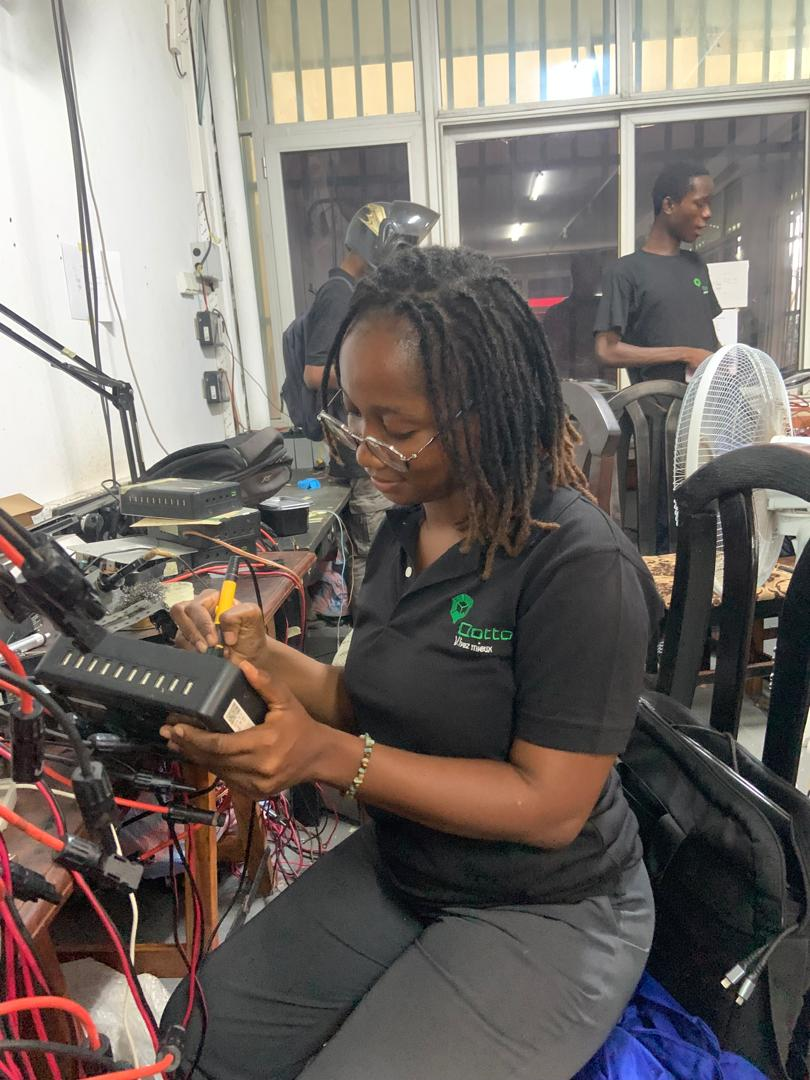
\includegraphics[width=\textwidth]{images/qotto_christelle.jpg}
        \caption{Christelle — diagnostic BMS}
    \end{subfigure}
    \hfill
    \begin{subfigure}[b]{0.47\textwidth}
        \centering
        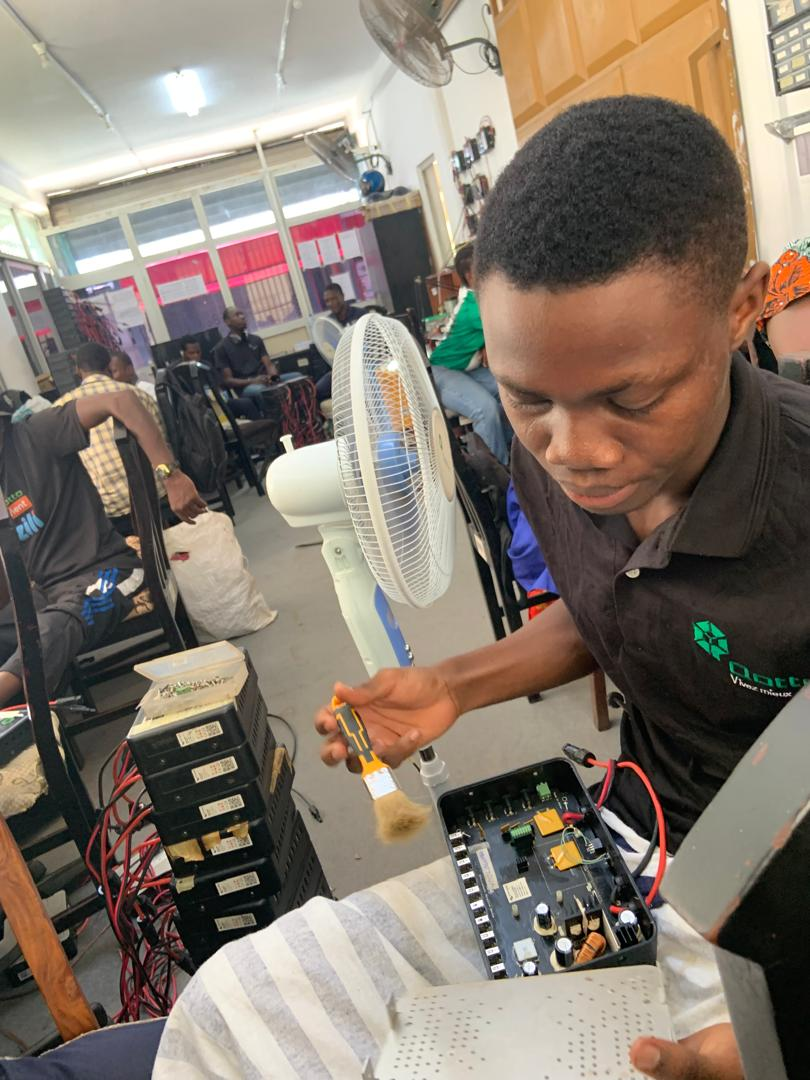
\includegraphics[width=\textwidth]{images/qotto_virgile.jpg}
        \caption{Virgile — reconditionnement}
    \end{subfigure}
    \caption{Les stagiaires en activité au sein de QOTTO Bénin}
    \label{fig:stagiaires_qotto}
\end{figure}
\FloatBarrier

\section{Déroulement des activités}
Afin d'appréhender l'ensemble des métiers de l'entreprise, une rotation hebdomadaire entre les différents postes techniques a été mise en place.

\subsection{Maintenance industrielle des systèmes solaires (BMS/Box)}
Le cœur de notre activité quotidienne a consisté à intervenir sur la chaîne de reconditionnement des BMS et des Box Qotto. Le processus industriel suit un flux rigoureux illustré par la Figure \ref{fig:flux_maintenance}.

\begin{figure}[H]
    \centering
    \begin{tikzpicture}[node distance=1.5cm, every node/.style={fill=white, font=\small}, align=center]
        % Styles
        \tikzstyle{process} = [rectangle, minimum width=5cm, minimum height=0.8cm, text centered, draw=ucaoBlue, fill=ucaoVeryLightBlue, line width=1pt, rounded corners]
        \tikzstyle{arrow} = [thick,->,>=stealth, ucaoBlue]
        
        % Nodes
        \node (start) [process] {1. Entrepôt : Réception, Acquisition et Répartition};
        \node (labo) [process, below of=start] {2. Laboratoire : Calibrage et Mises à jour};
        \node (test1) [process, below of=labo] {3. Poste Test Niveau 1 : Clavier, Ports, Activation};
        \node (rep1) [process, below of=test1] {4. Poste Réparation Niveau 1 (Clavier, Écran, Micro-contrôleur)};
        \node (rep2) [process, below of=rep1] {5. Poste Réparation Niveau 2 (Résistances, Ports)};
        \node (nonreg) [process, below of=rep2] {6. Poste Test de Non-régression};
        \node (recond) [process, below of=nonreg] {7. Reconditionnement : Nettoyage et Fermeture};

        % Arrows
        \draw [arrow] (start) -- (labo);
        \draw [arrow] (labo) -- (test1);
        \draw [arrow] (test1) -- (rep1);
        \draw [arrow] (rep1) -- (rep2);
        \draw [arrow] (rep2) -- (nonreg);
        \draw [arrow] (nonreg) -- (recond);
    \end{tikzpicture}
    \caption{Chaîne opérationnelle de reconditionnement des équipements QOTTO}
    \label{fig:flux_maintenance}
\end{figure}

L'organisation repose sur une rotation hebdomadaire des stagiaires entre les différents postes clés :
\begin{itemize}
    \item \textbf{Flux initial (Entrepôt) :} Après la réception, chaque BMS subit une phase d'acquisition de données. Les équipements sont ensuite répartis par catégories de pannes (problème panneau, clavier déprogrammé, etc.) avant leur transfert au laboratoire.
    \item \textbf{Traitement au Laboratoire :} Cette étape est dédiée au calibrage des BMS et à la mise à jour logicielle des systèmes.
    \item \textbf{Poste Test de Niveau 1 :} On y vérifie l'intégrité des claviers et des ports, suivie de la procédure d'activation. En cas de défaut, l'unité est orientée vers les postes de réparation.
    \item \textbf{Ateliers de Réparation (Niveau 1 et 2) :} Le niveau 1 traite les pannes d'interface (micro, écran, clavier). Le niveau 2 gère les problèmes de ports USB/DC et les alertes critiques nécessitant le remplacement de résistances ou de composants de puissance.
    \item \textbf{Contrôle et Clôture :} Chaque unité réparée subit un test de non-régression au "Poste 2" avant de rejoindre le reconditionnement pour le nettoyage final et la fermeture.
\end{itemize}

\subsection{Recherche et Développement (RD)}
Nous avons également collaboré avec le pôle RD sur les aspects liés à l'ingénierie système :
\begin{itemize}
    \item \textbf{Dimensionnement énergétique :} Apprentissage des méthodes de calcul (sous Google Sheets) pour la constitution d'offres de kits solaires adaptés aux besoins des clients (évaluation de la consommation pour des solutions allant de 3~kW à 5~kW).
    \item \textbf{Validation technologique :} Test de nouveaux kits et solutions innovantes avant leur déploiement massif sur le terrain béninois.
\end{itemize}

\subsection{Application des compétences au projet SMART-SOJA}
Le projet SMART-SOJA constitue la synthèse opérationnelle de notre stage, résultant d'une convergence de compétences acquises au sein de l'écosystème QOTTO. Le diagnostic électronique quotidien sur les BMS a directement renforcé notre capacité à concevoir et déboguer le circuit imprimé du prototype. L'expertise en dimensionnement énergétique obtenue au pôle RD a été transposée pour dimensionner l'alimentation photovoltaïque autonome du projet (panneau 50~W, batterie 12~V/20~Ah, régulateur MPPT). Enfin, l'utilisation des outils de laboratoire (station de soudure, matériel de test) a permis une réalisation physique aux standards professionnels. Cette synergie a permis d'ancrer notre travail académique dans une réalité industrielle concrète.

\section{Bilan du stage et compétences acquises}
Ce stage a permis de développer un ensemble de compétences techniques directement mobilisées dans la réalisation du projet SMART-SOJA :
\begin{itemize}
    \item \textbf{Diagnostic et réparation électronique :} Intervention sur les BMS et Box Qotto (Niveau 1 et 2), compétence réinvestie dans la conception et le débogage du PCB SMART-SOJA.
    \item \textbf{Dimensionnement énergétique :} Calcul de systèmes solaires de 3 à 5~kW, compétence appliquée au dimensionnement de l'alimentation photovoltaïque autonome du prototype.
    \item \textbf{Programmation embarquée :} Mise à jour logicielle et calibrage des systèmes Qotto, compétence transférée au développement du firmware FreeRTOS de l'ESP32.
    \item \textbf{Travail en équipe et documentation :} Suivi de la chaîne de maintenance, rédaction de rapports d'intervention, compétences mises à profit pour la documentation technique du projet.
\end{itemize}

\section{Difficultés rencontrées}
Le déroulement du stage a été marqué par plusieurs contraintes techniques et logistiques :
\begin{itemize}
    \item \textbf{Approvisionnement en composants :} Délais importants pour l'obtention de certains composants électroniques (capteurs, MOSFETs de puissance), accentués par des contraintes budgétaires.
    \item \textbf{Conception mécanique :} Complexité de la modélisation 3D complète du châssis modulaire sous SolidWorks, nécessitant plusieurs itérations.
    \item \textbf{Calibration des capteurs :} Ajustement des sondes d'humidité capacitives pour une mesure fiable sur les grains de soja, en l'absence d'hygromètre de référence certifié au laboratoire.
    \item \textbf{Intégration mécatronique :} Coordination entre les sous-systèmes mécaniques, électroniques et logiciels lors de l'assemblage final du prototype.
\end{itemize}

\section*{Synthèse et transition}
Ce chapitre a présenté le cadre institutionnel du stage effectué au sein de QOTTO Bénin, ainsi que les missions, les activités et les compétences techniques mobilisées durant cette immersion professionnelle. L'expérience acquise en diagnostic électronique, en dimensionnement énergétique et en programmation embarquée au sein de l'entreprise a directement nourri la conception du prototype SMART-SOJA, tandis que les difficultés rencontrées sur le terrain ont orienté certains choix techniques retenus par la suite. Fort de ce cadre pratique et des compétences ainsi consolidées, le chapitre suivant présente l'étude complète de la solution proposée, depuis l'analyse du contexte de la filière soja jusqu'à la réalisation du prototype.
